\section{Kolmogorov-Arnold representation theorem}
\label{sec:ka}
Whereas Multi-layer perceptrons (MLPs) are inspired by the universal approximation theorem, Kolmogorov-Arnold Networks (KANs) are inspired by the Kolmogorov-Arnold representation theorem \cite{KAN}.

Firstly, we start with the basic concept that a neural network can be described as a multivariate continuous function $f: \Re^n \rightarrow \Re^m $ that maps an input vector $\textbf{x}\in \Re^n$ to an output vector $\textbf{y}\in \Re^m$ via a series of computations. In particular, both MLPs and KANs can be described as a multivariate continuous function $f: \Re^n \rightarrow \Re $ that maps an input vector $\textbf{x}\in \Re^n$ to an output value $y\in \Re$ via a series of computations: $f(x) \equiv KAN(x)$ \cite{book1NAML, book2NAML}.

As in MLP when input variables are combined linearly we have to standardize inputs passing from a domain $D \subset \Re^n$ to a compact domain $D \subset [0,1]^n $. A possibility is to apply an affine transformation to the data so that each feature will be normalized in $[0,1] \in 
 \Re$.

\subsection{Theorem}
We can now formally present and demonstrate the Kolmogorov-Arnold representation theorem. 

The Kolmogorov-Arnold representation theorem is essential for proving that any neural network that has one output (for instance MLPs) can always be rebuilt as two-hidden-layer KANs. In particular, the Kolmogorov-Arnold representation theorem states that if $f$ is a multivariate continuous function on a bounded domain, then it can be written as a finite composition of continuous functions of a single variable and the binary operation of addition \cite{KAtheorem, KArevisited}.

\begin{theorem}[Kolmogorov-Arnold representation theorem \cite{KAtheorem}] 
\label{Kolmogorov-Arnold}
Let $f$ be an arbitrary multivariate continuous function on a bounded domain $f:[0,1]^n -> \Re$, then $f$:

$$f(\textbf{x}) = f(x_1,x_2,...,x_n) = \sum_{q=1}^{2n+1} \Phi_q(\sum_{p=1}^n \phi_{q,p}(x_p))$$

with continuous one–dimensional inner functions $\phi_{q,p}:[0,1] -> \Re$ and continuous one–dimensional outer functions $\Phi_q:\Re -> \Re$.
\end{theorem} 

In a sense, they showed that the only true multivariate function is addition since every other function can be written using univariate functions and sum. The great advantage is that we have to learn only a polynomial number of 1D functions. However, these 1D functions can be non-smooth and even fractal, so they may not be learnable; in practice with spline function, we can approximate their shapes and achieve the accuracy that we want \cite{KAN}.

\subsection{KAN matrix form}
\label{sec:ma}
For a more formal definition, we define the representation matrix of the Kolmogorov-Arnold representation theorem ( $f: [0,1]^n \rightarrow \Re$ ) \cite{KAN}:

$$f(\textbf{x}) = \boldsymbol{\Phi_{out}} \times \boldsymbol{\Phi_{in} }\times \textbf{x}$$

where $\textbf{x} \in \Re^n$, $\boldsymbol{\Phi_{in}} \in \Re^{2n+1,n}$, and $\boldsymbol{\Phi_{out}} \in \Re^{2n+1}$:

\[
\boldsymbol{\Phi_{in}} = 
\begin{pmatrix}
\phi_{1,1}(\cdot) & \dots & \phi_{1,n}(\cdot) \\
\vdots &   & \vdots \\
\phi_{2n+1,1}(\cdot) & \dots & \phi_{2n+1,n}(\cdot)
\end{pmatrix},
\quad \boldsymbol{\Phi_{out}} = (\Phi_{1}(\cdot) \dots \Phi_{2n+1}(\cdot))
\]

\begin{figure}[H]
    \centering
    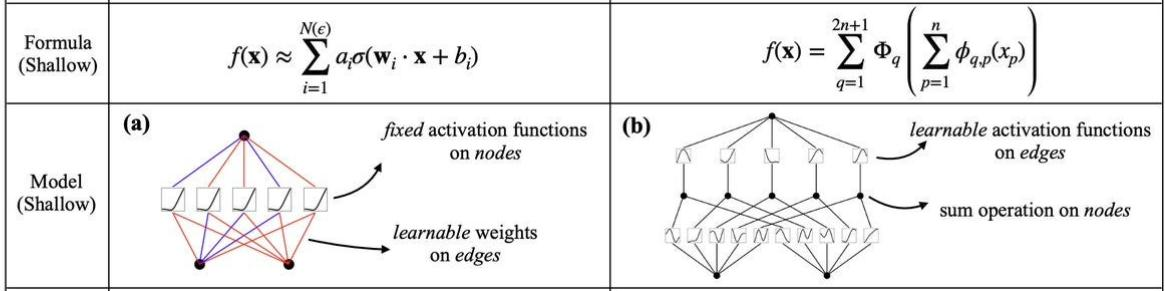
\includegraphics[width=0.8\linewidth]{Images/A.JPG}
    \caption{ MLPs vs KANs: Shallow model}
\end{figure}

\subsubsection{KAN layer form}
We notice that both matrices $\boldsymbol{\Phi_{in}}$ and $\boldsymbol{\Phi_{out}}$ are special cases of the matrix $\boldsymbol{\Phi} \in \Re^{n_{out},n_{in}}$ that represent a general Kolmogorov-Arnold layer. 

\[
\boldsymbol{\Phi} = 
\begin{pmatrix}
\phi_{1,1}(\cdot) & \dots & \phi_{1,n_{in}}(\cdot) \\
\vdots &   & \vdots \\
\phi_{n_{out},1}(\cdot) & \dots & \phi_{n_{out},n_{in}}(\cdot)
\end{pmatrix} 
\]

so each layer map his input $l$ $\textbf{x}_l$ to the output $\textbf{x}_{l+1}$ thought $\boldsymbol{\Phi}$:

\[
\textbf{x}_{l+1} = \boldsymbol{\Phi} \times \textbf{x}_l \Rightarrow
\textbf{x}_{l+1} = 
\begin{pmatrix}
\phi_{1,1}(\cdot) & \dots & \phi_{1,n_{in}}(\cdot) \\
\vdots &   & \vdots \\
\phi_{n_{out},1}(\cdot) & \dots & \phi_{n_{out},n_{in}}(\cdot)
\end{pmatrix} \textbf{x}_l
\]


Each layer has $n_{in}$ inputs and $n_{out}$ outputs and is mapped thought its respective layer matrix. In our case, the two layers are defined as follows:
\begin{itemize}
    \item Layer 1: $\boldsymbol{\Phi_{in}}$ has $\boldsymbol{\Phi}$ with $n_{in} = n$ and $n_{out} = 2n+1$
    \item Layer 2: $\boldsymbol{\Phi_{out}}$ has $\boldsymbol{\Phi}$ with $n_{in} = 2n+1$ and $n_{out} = 1$
\end{itemize}